\subsection{Code generator}
As soon as a language is defined, for example by writing it down in \ac{EBNF}, the development of a code generator can be started. Generators can be implemented using a template-based approach \parencite[see][]{cleaveland_program_2001}, the template metaprogramming capabilities of a language (e.g., in C++), or extendable programming systems (e.g., OpenC++) \parencite[cf.][p. 16]{czarnecki_generative_2000}.\\
A code generator generally consists of several different phases or components, as shown in the following figure.
\begin{figure}[H]
    \caption{Code Generation Processing Phases}
    \label{fig:generator-process}
    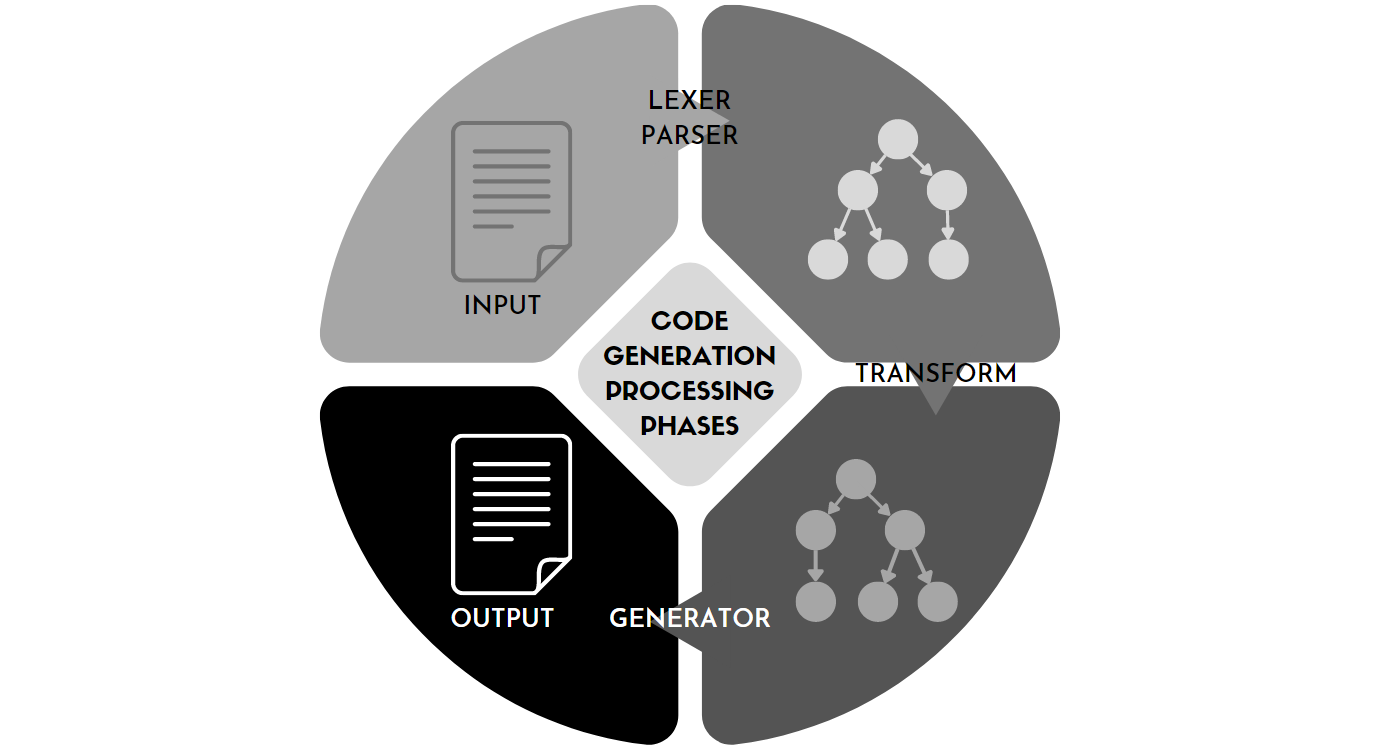
\includegraphics[width=0.9\textwidth]{generator-process.png}
    \\
    \cite[Source: Based on][p. 5]{sarkar_code_2001}
\end{figure}
A program written by a developer in either a predefined \ac{DSL} or an executable model is stored in a file for development. The code generator is given the grammar of the source language, which it uses to split it into tokens and then relate them to each other by parsing them. Such dependencies can also exist between multiple input files, by importing or referencing each other. The parser then arranges them in an \ac{AST}, which can be optimized and transformed for the target language. The generator or writer then generates a file in the target language from this \ac{AST}.